\documentclass[aspectratio=169]{beamer}
\usetheme{Madrid}
\usecolortheme{seahorse}
\usepackage{tikz}
\usepackage{fontawesome5}
\usepackage{booktabs}
\usepackage{listings}
\usepackage{xcolor}

% Custom colors
\definecolor{localgreen}{RGB}{0,212,170}
\definecolor{cloudred}{RGB}{255,107,107}
\definecolor{cacheyellow}{RGB}{255,217,61}
\definecolor{darkbg}{RGB}{26,26,46}
\definecolor{codebg}{RGB}{22,33,62}

\setbeamercolor{frametitle}{bg=darkbg,fg=white}
\setbeamercolor{title}{fg=white}
\setbeamercolor{author}{fg=white}
\setbeamercolor{date}{fg=white}
\setbeamertemplate{navigation symbols}{}

\lstset{
  basicstyle=\ttfamily\footnotesize,
  backgroundcolor=\color{codebg},
  keywordstyle=\color{localgreen}\bfseries,
  commentstyle=\color{gray},
  stringstyle=\color{cacheyellow},
  breaklines=true,
  frame=single,
  rulecolor=\color{gray},
  xleftmargin=5pt,
  xrightmargin=5pt,
}

\title{\textbf{Inference RIC Pipeline}}
\subtitle{Router $\rightarrow$ Inference $\rightarrow$ Cache\\
Mac Mini M3 + Gemma 3 + OmniRoute}
\author{Lab AI Infrastructure Team}
\date{\today}

\begin{document}

% ── Title Slide ────────────────────────────────
\begin{frame}
\titlepage
\end{frame}

% ── Outline ───────────────────────────────────
\begin{frame}{Outline}
\tableofcontents
\end{frame}

% ── Section 1 ─────────────────────────────────
\section{Problem \& Motivation}

\begin{frame}{Why Do We Need RIC?}
\begin{columns}
\column{0.5\textwidth}
\textbf{\color{cloudred}Current Problems:}
\begin{itemize}
  \item All queries go to cloud API
  \item High token consumption = high cost
  \item Network latency for simple queries
  \item API rate limits slow down research
  \item Repeated queries re-charged every time
\end{itemize}
\column{0.5\textwidth}
\textbf{\color{localgreen}RIC Solution:}
\begin{itemize}
  \item Simple queries $\rightarrow$ \textbf{Mac Mini (free)}
  \item Complex queries $\rightarrow$ Cloud (only when needed)
  \item Repeated queries $\rightarrow$ \textbf{Cache (instant)}
  \item Estimated \textbf{60--80\% token reduction}
  \item Faster responses for routine tasks
\end{itemize}
\end{columns}
\end{frame}

% ── Section 2 ─────────────────────────────────
\section{System Architecture}

\begin{frame}{RIC Architecture Overview}
\begin{center}
\begin{tikzpicture}[
  node distance=1.5cm,
  box/.style={rectangle, rounded corners, minimum width=2.2cm, minimum height=0.8cm,
              text centered, font=\bfseries\small},
  arr/.style={->, thick, >=stealth}
]
  \node[box, fill=white!20, draw=white] (user) {User Query};

  \node[box, fill=blue!70, draw=blue!30, below of=user] (cache) {\faDatabase\; Cache Check};

  \node[box, fill=purple!70, draw=purple!30, below of=cache] (router) {\faCodeBranch\; Router};

  \node[box, fill=localgreen!80, draw=localgreen, left=2cm of router] (local)
    {\faApple\; Mac Mini M3\\Gemma 3 12B};

  \node[box, fill=cloudred!80, draw=cloudred, right=2cm of router] (cloud)
    {\faCloud\; OmniRoute\\Cloud API};

  \node[box, fill=cacheyellow!60, draw=cacheyellow, below=1.8cm of router] (store)
    {\faHdd\; Store in Cache};

  \draw[arr, white] (user) -- (cache) node[midway, right, white, font=\tiny] {query};
  \draw[arr, cacheyellow] (cache) -- node[right, font=\tiny, white]{MISS} (router);
  \draw[arr, cacheyellow, bend right=60] (cache) to node[left, font=\tiny, cacheyellow]{HIT (instant!)} (store);
  \draw[arr, localgreen] (router) -- node[above, font=\tiny, white]{simple} (local);
  \draw[arr, cloudred] (router) -- node[above, font=\tiny, white]{complex} (cloud);
  \draw[arr, white] (local) |- (store);
  \draw[arr, white] (cloud) |- (store);
\end{tikzpicture}
\end{center}
\end{frame}

\begin{frame}{Hardware \& Software Stack}
\begin{columns}
\column{0.5\textwidth}
\textbf{Hardware: Mac Mini M3}
\begin{itemize}
  \item Apple M3 chip (Neural Engine)
  \item Unified Memory (16/24 GB)
  \item 512 GB SSD storage
  \item Always-on local inference server
  \item 0 API cost per inference
\end{itemize}
\vspace{0.3cm}
\textbf{Local Model: Gemma 3 12B (4-bit)}
\begin{itemize}
  \item Google's Gemma 3 via Ollama
  \item 4-bit quantized = fits in 8GB RAM
  \item Fast inference on Apple Silicon
  \item Good quality for routine tasks
\end{itemize}
\column{0.5\textwidth}
\textbf{Software Stack:}
\begin{itemize}
  \item \textbf{Ollama} — local model server
  \item \textbf{FastAPI} — RIC pipeline API
  \item \textbf{SQLite} — async cache (aiosqlite)
  \item \textbf{httpx} — async HTTP calls
  \item \textbf{Python 3.11+} — core language
\end{itemize}
\vspace{0.3cm}
\textbf{Cloud Backend:}
\begin{itemize}
  \item OmniRoute gateway
  \item Claude / GLM fallback models
  \item Only activated for complex tasks
\end{itemize}
\end{columns}
\end{frame}

% ── Section 3 ─────────────────────────────────
\section{Routing Logic}

\begin{frame}{How the Router Works}
\begin{block}{Routing Decision Flow}
\begin{enumerate}
  \item \textbf{Cache check first} — if seen before, return instantly (0 tokens)
  \item \textbf{Keyword match} — cloud keywords trigger cloud routing
  \item \textbf{Word count} — queries $\leq 60$ words $\rightarrow$ local
  \item \textbf{Fallback} — complex/long queries $\rightarrow$ cloud
\end{enumerate}
\end{block}

\vspace{0.3cm}
\begin{columns}
\column{0.5\textwidth}
\textbf{\color{localgreen}$\rightarrow$ LOCAL (Mac Mini)}
\begin{itemize}
  \item ``What is photosynthesis?''
  \item ``Define machine learning''
  \item ``Translate hello to French''
  \item ``List 5 Python libraries''
\end{itemize}
\column{0.5\textwidth}
\textbf{\color{cloudred}$\rightarrow$ CLOUD (OmniRoute)}
\begin{itemize}
  \item ``Write code for a federated learning system...''
  \item ``Analyze the architecture differences between...''
  \item ``Debug this Python code and explain step by step...''
  \item ``Research and compare GPT-4 vs Claude 3...''
\end{itemize}
\end{columns}
\end{frame}

% ── Section 4 ─────────────────────────────────
\section{Cache System}

\begin{frame}{Cache Layer Design}
\begin{columns}
\column{0.55\textwidth}
\textbf{SQLite Cache (aiosqlite)}
\begin{itemize}
  \item \textbf{Key}: MD5 hash of normalized query
  \item \textbf{TTL}: 24 hours (configurable)
  \item \textbf{Max entries}: 10,000
  \item \textbf{LRU eviction} when limit reached
  \item Stores: response, destination, tokens, latency
  \item Auto-clears expired entries on startup
\end{itemize}
\vspace{0.3cm}
\textbf{Cache Benefits:}
\begin{itemize}
  \item[\color{cacheyellow}$\star$] \textbf{0 tokens consumed} on cache hit
  \item[\color{cacheyellow}$\star$] \textbf{$<$5ms latency} vs 1000ms+ cloud
  \item[\color{cacheyellow}$\star$] Works offline (local cache)
  \item[\color{cacheyellow}$\star$] Shared across all lab members
\end{itemize}
\column{0.45\textwidth}
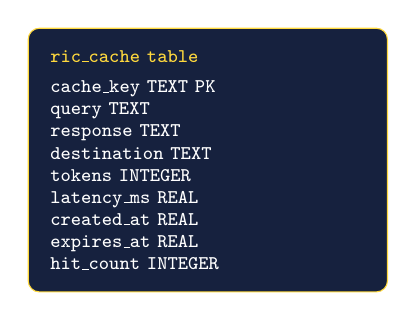
\begin{tikzpicture}
  \node[rectangle, draw=cacheyellow, fill=codebg, rounded corners,
        text width=4cm, font=\ttfamily\scriptsize, text=white,
        inner sep=8pt] {
    \textbf{\color{cacheyellow}ric\_cache table} \\[3pt]
    cache\_key TEXT PK \\
    query TEXT \\
    response TEXT \\
    destination TEXT \\
    tokens INTEGER \\
    latency\_ms REAL \\
    created\_at REAL \\
    expires\_at REAL \\
    hit\_count INTEGER
  };
\end{tikzpicture}
\end{columns}
\end{frame}

% ── Section 5 ─────────────────────────────────
\section{API \& Usage}

\begin{frame}[fragile]{FastAPI Server Endpoints}
\begin{lstlisting}[language=bash]
# Start the RIC server
python server.py
# Server runs on http://0.0.0.0:8000

# Run a query through the pipeline
curl -X POST http://localhost:8000/infer \
  -H "Content-Type: application/json" \
  -d '{"query": "What is photosynthesis?"}'

# Check health (local + cloud connectivity)
curl http://localhost:8000/health

# Get cache + routing statistics
curl http://localhost:8000/stats

# Clear cache
curl -X DELETE http://localhost:8000/cache/clear
\end{lstlisting}
\vspace{0.2cm}
\textbf{Swagger UI:} \texttt{http://localhost:8000/docs}
\end{frame}

\begin{frame}[fragile]{Python API Usage}
\begin{lstlisting}[language=Python]
from ric.pipeline import RICPipeline
import asyncio

async def main():
    pipeline = RICPipeline()
    await pipeline.init()

    # Simple query → automatically routed to Mac Mini
    result = await pipeline.run("What is photosynthesis?")
    print(result.destination)   # "local"
    print(result.latency_ms)    # ~800ms

    # Same query again → cache hit!
    result2 = await pipeline.run("What is photosynthesis?")
    print(result2.destination)  # "cache"
    print(result2.latency_ms)   # ~2ms  (instant!)

    # Complex query → routed to cloud
    result3 = await pipeline.run("Write a federated learning system...")
    print(result3.destination)  # "cloud"

asyncio.run(main())
\end{lstlisting}
\end{frame}

% ── Section 6 ─────────────────────────────────
\section{Benchmark Results}

\begin{frame}{Expected Performance (Mac Mini M3)}
\begin{table}
\centering
\begin{tabular}{lrrrl}
\toprule
\textbf{Backend} & \textbf{Avg Latency} & \textbf{Tokens/Query} & \textbf{Cost} & \textbf{Best For} \\
\midrule
\color{localgreen}Local (Gemma M3)  & 800--2000ms & $\sim$200    & \color{localgreen}\$0.00 & Simple queries \\
\color{cloudred}Cloud (OmniRoute)   & 1500--4000ms & $\sim$800   & \color{cloudred}\$\$    & Complex tasks \\
\color{cacheyellow}Cache (SQLite)   & 1--5ms      & \textbf{0}   & \color{cacheyellow}\$0.00 & Repeated queries \\
\midrule
\textbf{RIC Pipeline}               & \textbf{Mixed} & \textbf{-60--80\%} & \textbf{Low} & \textbf{All queries} \\
\bottomrule
\end{tabular}
\end{table}

\vspace{0.3cm}
\begin{block}{Token Reduction Breakdown}
\begin{itemize}
  \item Simple queries (local): \textbf{100\% cloud token saving}
  \item Repeated queries (cache): \textbf{100\% token saving}
  \item Complex queries: \textbf{0\% saving} (unavoidable)
  \item Overall estimated reduction: \textbf{60--80\% depending on workload}
\end{itemize}
\end{block}
\end{frame}

% ── Section 7 ─────────────────────────────────
\section{Setup Guide}

\begin{frame}[fragile]{Setup: Mac Mini (Step 1 of 3)}
\begin{block}{Install Ollama and pull Gemma 3}
\begin{lstlisting}[language=bash]
# On Mac Mini — install Ollama
brew install ollama

# Pull Gemma 3 12B (best for M3 with 16GB RAM)
ollama pull gemma3:12b

# Or Gemma 3 4B (for 8GB RAM Mac Mini)
ollama pull gemma3:4b

# Start Ollama server (runs on port 11434)
ollama serve

# Verify it works
curl http://localhost:11434/api/generate \
  -d '{"model":"gemma3:12b","prompt":"Hello!","stream":false}'
\end{lstlisting}
\end{block}
\textit{Ollama auto-starts on Mac login. Gemma3:12b uses $\sim$8GB unified memory.}
\end{frame}

\begin{frame}[fragile]{Setup: RIC Pipeline (Step 2 of 3)}
\begin{block}{Install and configure RIC}
\begin{lstlisting}[language=bash]
# Clone / navigate to project
cd /home/crypto_nn/ric_inference

# Create virtual environment and install
python3 -m venv venv && source venv/bin/activate
pip install -r requirements.txt

# Edit config.yaml — set your IPs
nano config.yaml
# Set: local.host = <mac-mini-ip>
# Set: cloud.base_url = <omni-route-ip>
# Set: cloud.api_key = <your-key>
\end{lstlisting}
\end{block}
\begin{block}{Edit config.yaml key fields}
\begin{lstlisting}[language=yaml]
local:
  host: "192.168.1.XXX"   # Mac Mini IP
  model: "gemma3:12b"
cloud:
  base_url: "http://YOUR_OMNI_ROUTE/v1"
  api_key: "YOUR_KEY"
\end{lstlisting}
\end{block}
\end{frame}

\begin{frame}[fragile]{Setup: Run \& Benchmark (Step 3 of 3)}
\begin{block}{Start the server and run benchmark}
\begin{lstlisting}[language=bash]
# Start the FastAPI server
python server.py
# → API available at http://localhost:8000
# → Docs at http://localhost:8000/docs

# Test a quick query
python client_example.py

# Run full benchmark (local vs cloud vs RIC)
python benchmark.py
# → Rich table in terminal
# → Chart saved: logs/benchmark_results.png
# → JSON report: logs/benchmark_report.json

# Health check
curl http://localhost:8000/health
\end{lstlisting}
\end{block}
\end{frame}

% ── Summary ───────────────────────────────────
\section{Summary}

\begin{frame}{Summary \& Contributions}
\begin{columns}
\column{0.5\textwidth}
\textbf{What We Built:}
\begin{enumerate}
  \item \textbf{Router} — keyword + word-count based routing
  \item \textbf{Local Inference} — Ollama + Gemma3 on M3
  \item \textbf{Cloud Inference} — OmniRoute API adapter
  \item \textbf{Cache Layer} — async SQLite with TTL + LRU
  \item \textbf{Pipeline} — orchestrates all 3 components
  \item \textbf{FastAPI Server} — REST API for lab use
  \item \textbf{Benchmark Script} — quantified comparisons
\end{enumerate}
\column{0.5\textwidth}
\textbf{Expected Benefits:}
\begin{itemize}
  \item[\color{localgreen}$\checkmark$] 60--80\% token cost reduction
  \item[\color{localgreen}$\checkmark$] Sub-5ms cache responses
  \item[\color{localgreen}$\checkmark$] Free local inference (M3)
  \item[\color{localgreen}$\checkmark$] Transparent to users
  \item[\color{localgreen}$\checkmark$] Easy to extend routing rules
  \item[\color{localgreen}$\checkmark$] Full logging \& monitoring
\end{itemize}
\vspace{0.3cm}
\textbf{Next Steps:}
\begin{itemize}
  \item Fine-tune routing threshold
  \item Add ML-based classifier router
  \item Redis cache for multi-node lab
\end{itemize}
\end{columns}
\end{frame}

\begin{frame}[plain]
\begin{center}
{\Huge \textbf{Thank You}}\\[1cm]
{\Large Questions?}\\[1cm]
\faGithub\ \texttt{/home/crypto\_nn/ric\_inference}\\[0.5cm]
\textbf{RIC Pipeline v1.0}\\
Mac Mini M3 · Gemma 3 12B · OmniRoute
\end{center}
\end{frame}

\end{document}
